% !TeX root = ta.tex
\cleardoublepage % memastikan bab baru dimulai di halaman ganjil (kanan)
\chapter{STUDI LITERATUR}
\label{chap:studi-literatur}
\section{Tumor Otak}
Berdasarkan \textcite{mayo2023brain}, tumor otak didefinisikan sebagai pertumbuhan abnormal sel yang terjadi di dalam atau di dekat otak. Lokasi tumor dapat bervariasi, mencakup jaringan otak, saraf, kelenjar pituitari, kelenjar pineal, serta membran yang menutupi permukaan otak. Tumor yang bermula di otak disebut tumor otak primer, sedangkan tumor yang menyebar ke otak dari bagian tubuh lain disebut tumor otak sekunder atau metastatik.

\subsection{Teknologi Pencitraan Medis Tumor Otak}

Langkah awal untuk mendiagnosis tumor otak adalah pemeriksaan fisik, tes penglihatan, riwayat medis, dan tes neurologis untuk mengevaluasi fungsi otak serta saraf. Jika tes awal menunjukkan kemungkinan adanya tumor otak, pencitraan diagnostik akan dilakukan dan dianalisis oleh ahli neuroradiologi \autocite{farber2025how}. Dalam pencitraan tumor otak, terdapat tiga bidang utama yang bisa dilakukan oleh alat pencitraan seperti pada Gambar \ref{gambar:gambartumor} \autocite{hartung2023abdominal}.

\begin{figure}[H]
	\centering
	\captionsetup{justification=centering}
	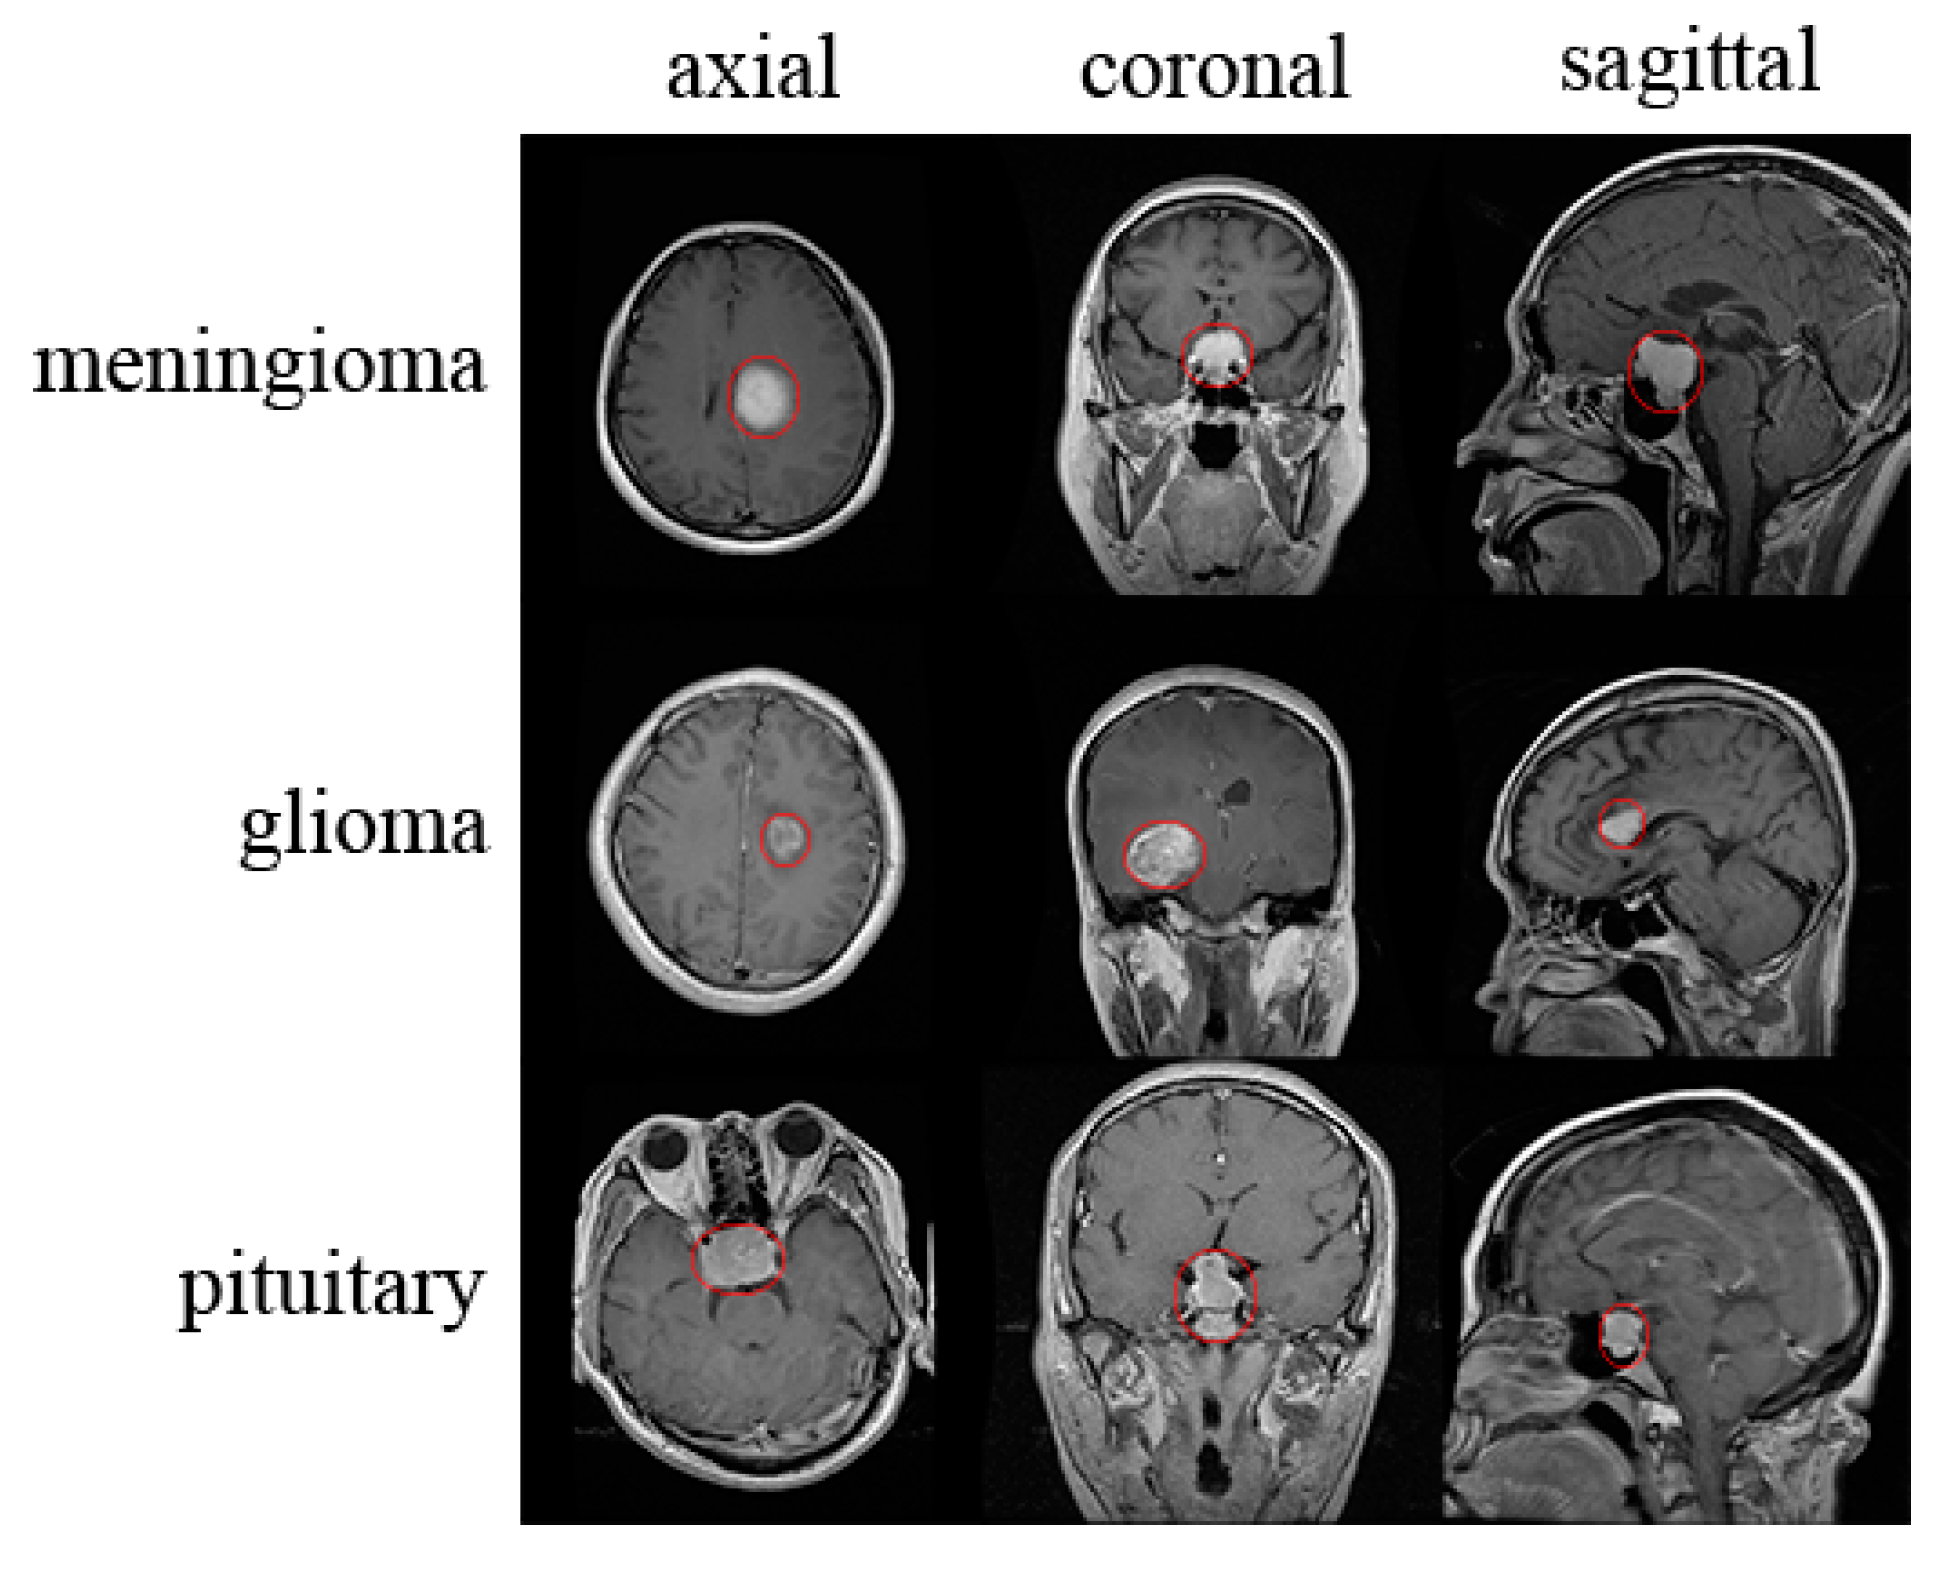
\includegraphics[width=0.6\textwidth]{images/gambartumor.png}
	\caption{\textit{CT Scan} Otak 
		\autocite{kamesh2024brain}}
	\label{gambar:gambartumor}
\end{figure}

Berdasarkan \textcite{radiologykey2015brain}, terdapat tiga bidang dalam pencitraan medis.
\begin{enumerate}
	
	\item Bidang Aksial\\
	Bidang aksial adalah bidang horizontal yang membagi tubuh menjadi bagian atas dan bawah, tegak lurus terhadap sumbu panjang tubuh. Dalam pencitraan medis seperti \textit{CT Scan}, bidang ini menampilkan irisan tubuh yang dilihat dari arah kaki menuju kepala atau sebaliknya.
	
	\item Bidang Koronal\\
	Bidang koronal adalah bidang vertikal yang membagi tubuh menjadi bagian depan dan belakang. Penamaannya merujuk pada \textit{coronal suture} tengkorak, yakni garis sambungan tulang yang melintang dari telinga kiri ke kanan, menyerupai letak mahkota atau bando.
	
	\item Bidang Sagital\\
	Bidang sagital adalah bidang vertikal yang membagi tubuh menjadi sisi kanan dan kiri. Penamaannya merujuk pada \textit{sagittal suture} tengkorak yang posisinya menyerupai arah anak panah jika dilihat dari depan.
\end{enumerate}

\subsubsection{MRI}
\textit{Magnetic Resonance Imaging} (MRI) merupakan teknologi pencitraan 3D noninvasif beresolusi tinggi yang memanfaatkan interaksi medan magnet kuat dan gelombang radio terhadap proton dalam molekul air pada jaringan tubuh. Berdasarkan perbedaan waktu relaksasi energi proton tersebut, MRI sangat unggul untuk memvisualisasikan detail anatomi jaringan lunak, seperti struktur otak, saraf, dan otot, serta efektif dalam mendiagnosis tumor tanpa paparan radiasi. Meskipun aman dari radiasi, penggunaannya dikontraindikasikan bagi pasien dengan implan logam (misalnya alat pacu jantung) dan memiliki risiko penyerta seperti kebisingan, stimulasi saraf, hingga potensi toksisitas agen kontras gadolinium pada penderita gangguan ginjal \autocite{nibib2025mri}.

\subsubsection{\textit{CT Scan}}
\textit{Computed Tomography} (CT) adalah prosedur pencitraan diagnostik yang menggunakan teknologi sinar-X. Prosedur ini bekerja dengan mengarahkan berkas sinar-X yang sempit dan berputar cepat mengelilingi tubuh pasien. Sinyal yang dihasilkan kemudian diproses oleh komputer untuk membuat serangkaian gambar irisan tomografi secara detail, yang dapat direkonstruksi menjadi gambar tiga dimensi (3D).

\textit{CT Scan} memiliki peran penting sebagai instrumen peringatan dini dalam mendiagnosis tumor otak. Berdasarkan penelitian oleh \textcite{budiman2024effectiveness}, penggunaan \textit{CT Scan} terbukti sangat efektif dan memberikan dampak positif bagi deteksi dini tumor otak pada manusia. Tingkat efektivitas ini dibuktikan secara kuantitatif melalui perolehan nilai rata-rata \textit{effect size} sebesar 1,17 yang masuk dalam kategori tinggi. Selain itu, hasil pengujian N-Gain juga menunjukkan skor 0,58 dengan kategori efektivitas tinggi.

Meskipun MRI sering dianggap sebagai metode pencitraan yang lebih sensitif dalam mendeteksi keberadaan tumor yang berukuran kecil, \textit{CT Scan} tetap menawarkan keunggulan lain, seperti tingkat ketersediaan alat yang lebih merata di berbagai fasilitas kesehatan serta waktu pemeriksaan yang jauh lebih singkat. Temuan yang mendukung efektivitas \textit{CT Scan} pada tahap awal ini berdampak besar pada praktik klinis sehari-hari. Modalitas dapat membuat proses pengambilan keputusan diagnostik dan perencanaan pengobatan pasien menjadi lebih cepat dan efektif.

\textit{CT Scan} dapat digunakan untuk mengidentifikasi penyakit atau cedera, seperti mencitrakan kepala untuk menemukan cedera, tumor, atau gumpalan yang menyebabkan \textit{stroke} serta mencitrakan paru-paru atau patah tulang yang kompleks. Di samping kelebihan yang dimiliki, \textit{CT Scan} juga memiliki kelemahan, yaitu penggunaan radiasi yang memiliki risiko biologis, serta agen kontras yang berpotensi menyebabkan reaksi alergi atau gangguan ginjal pada pasien tertentu \autocite{nibib2022ct}.

\begin{figure}[H]
	\centering
	\captionsetup{justification=centering}
	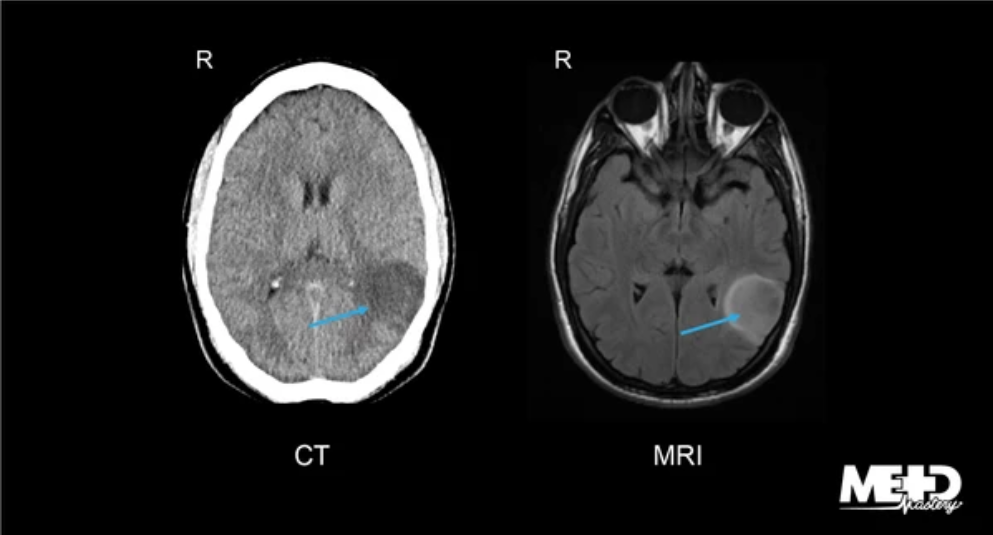
\includegraphics[width=0.7\textwidth]{images/ctvsmri.png}
	\caption{Perbandingan \textit{CT Scan} dan MRI Otak 
		\autocite{mamourian2020recognizing}}
	\label{gambar:ctvsmri}
\end{figure}

Selain risiko biologis, \textit{CT Scan} juga kurang sensitif dalam mendiagnosis, seperti yang terlihat pada Gambar \ref{gambar:ctvsmri}. Pada kasus tumor \textit{intra-axial}, masalah utamanya adalah kurang jelasnya gambar jaringan lunak. Menurut \textcite{mamourian2020recognizing}, banyak tumor jenis ini bersifat \textit{isodense} atau kepadatannya mirip dengan jaringan otak normal. Akibatnya, tumor sulit dibedakan jika tidak memakai cairan kontras atau dibandingkan dengan hasil MRI. Selain itu, sering terjadi kebingungan diagnosis karena tumor bisa terlihat seperti penyakit lain, seperti infark subakut, abses otak, atau lesi demielinisasi. Masalah ini bisa diperparah oleh bias konfirmasi, seperti pembacaan hasil \textit{CT Scan} terpengaruh oleh riwayat penyakit pasien. Oleh karena itu, kunci untuk mendeteksi tumor \textit{intra-axial} pada \textit{CT Scan} adalah dengan mengamati tanda-tanda kecil lainnya secara teliti \autocite{mamourian2020recognizing}.

\section{\textit{Artificial Intelligence} (AI) dalam Pencitraan Medis}
Implementasi AI pada citra medis memiliki dampak besar pada berbagai tugas dalam alur kerja radiologi. AI berdampak pada tugas-tugas klinis berbasis gambar, seperti deteksi kelainan, karakterisasi objek dalam gambar menggunakan segmentasi, diagnosis, dan penentuan stadium, serta pemantauan objek untuk diagnosis dan penilaian respons pengobatan.

Dalam konteks transparansi dan kemampuan interpretasi keputusan medis, model-model pembelajaran mesin tersebut dapat dikategorikan lebih lanjut menjadi dua jenis utama \autocite{moreira2024benchmarking}:

\begin{enumerate}
	\item \textit{White-Box Models} \\
	Model ini dirancang dengan logika dasar dan proses yang jelas, sehingga mekanisme pengambilan keputusannya secara dapat ditafsirkan oleh manusia. Pengguna dapat memahami bagaimana model bekerja dengan memeriksa struktur internalnya secara langsung, seperti melihat bobot fitur atau aturan keputusan. Contoh algoritma yang termasuk dalam kategori ini adalah \textit{Decision Trees} dan regresi linier.
	
	\item \textit{Black-Box Models} \\
	Model ini memiliki mekanisme internal yang sangat kompleks sehingga sulit atau tidak mungkin bagi pengguna manusia untuk memahami bagaimana prediksi atau hasil spesifik dihasilkan. Karena kompleksitasnya, hubungan antara \textit{input} dan \textit{output} sering dianggap sebagai misteri yang tidak dapat diperiksa secara manual. \textit{Deep Neural Networks} dan model \textit{ensemble} yang rumit merupakan representasi utama dari kategori ini.
\end{enumerate}

Terdapat dua metode utama dalam pencitraan medis untuk tugas klasifikasi seperti membedakan tumor jinak atau ganas, yaitu \textit{machine learning} tradisional dan \textit{deep learning} \autocite{hosny2018artificial}.

\subsection{\textit{Deep Learning}}
\textit{Deep learning} menggunakan sistem \textit{layers} yang secara bersamaan melakukan ekstraksi fitur, seleksi, dan klasifikasi selama proses pelatihan. Lapisan-lapisan ini belajar mengenali fitur dari yang abstrak, seperti garis hingga yang kompleks, seperti organ \autocite{hosny2018artificial}. Beberapa teknik utama yang biasa digunakan, yaitu:

\begin{enumerate}
	\item CNN (\textit{Convolutional Neural Networks})
	
	CNN adalah model \textit{deep learning} yang dirancang untuk memproses data dengan topologi seperti \textit{grid} dengan contoh berupa gambar. CNN dapat digunakan untuk mendeteksi objek dalam gambar seperti orang, mobil, dan bangunan. CNN juga dapat digunakan untuk melokalisasi objek dalam gambar, yang berarti dapat mengidentifikasi lokasi suatu objek dalam gambar. 
	
	CNN memiliki beberapa komponen kunci. Pertama, \textit{convolutional layers} yang menerapkan filter pada gambar masukan untuk mendeteksi fitur seperti tepi dan tekstur, sekaligus menjaga hubungan spasial antarpiksel. Kedua, \textit{pooling layers} yang melakukan pengurangan sampel untuk mengurangi kompleksitas komputasi dan jumlah parameter. Ketiga, \textit{activation functions} yang memperkenalkan nonlinieritas agar model dapat mempelajari hubungan data yang kompleks. Terakhir, \textit{fully connected layers} yang bertanggung jawab membuat prediksi akhir berdasarkan fitur yang telah dipelajari oleh lapisan-lapisan sebelumnya \autocite{gfg2020cnn}. 
	
\end{enumerate}

\subsection{\textit{Transfer Learning}}
\label{subsec:transferlearning}
\textit{Transfer learning} adalah salah satu pendekatan dalam pembelajaran mesin yang memungkinkan sebuah model memanfaatkan pengetahuan yang sudah didapatkan dari suatu permasalahan (disebut domain sumber) untuk membantu menyelesaikan permasalahan lain yang masih berkaitan (disebut domain target) \cite{zhuang2020comprehensive}. Ide dasarnya cukup sederhana, yaitu daripada melatih model dari nol menggunakan data domain target yang jumlahnya terbatas, pengetahuan yang sudah dipelajari model dari domain sumber (yang biasanya memiliki data lebih banyak) dapat digunakan kembali. Dengan cara ini, kebutuhan data berlabel pada domain target dapat berkurang.

Berbeda dengan pembelajaran mesin konvensional yang mengasumsikan data latih dan data uji berasal dari distribusi yang sama, pada \textit{transfer learning} domain sumber dan domain target boleh memiliki distribusi data yang berbeda \cite{zhuang2020comprehensive}. Secara sederhana, sebuah domain dapat dipahami sebagai kombinasi antara ruang fitur (jenis data yang digunakan) dan distribusi datanya, sedangkan \textit{task} adalah kombinasi antara ruang label dan fungsi yang digunakan untuk memprediksi label tersebut.

Berdasarkan kesesuaian ruang fitur dan ruang label antara domain sumber dan domain target, \textit{transfer learning} dapat dibedakan menjadi dua jenis, yaitu:
\begin{enumerate}
	\item \textit{Homogeneous transfer learning}, yaitu ketika domain sumber dan domain target memiliki jenis fitur dan label yang sama, sehingga proses adaptasinya menjadi lebih sederhana.
	\item \textit{Heterogeneous transfer learning}, yaitu ketika ruang fitur atau ruang label antara kedua domain berbeda, sehingga dibutuhkan tahap tambahan untuk menyamakan representasi fitur sebelum pengetahuan dapat ditransfer \cite{zhuang2020comprehensive}.
\end{enumerate}

Menurut \cite{zhuang2020comprehensive}, pendekatan-pendekatan \textit{transfer learning} yang telah dikembangkan secara garis besar dapat dikelompokkan menjadi dua sudut pandang, yaitu:
\begin{enumerate}
	\item Pendekatan berbasis data (\textit{data-based}), yang berfokus pada penyesuaian data itu sendiri, misalnya dengan memberi bobot pada data domain sumber agar distribusinya menyerupai domain target, atau dengan mentransformasikan fitur ke representasi baru yang lebih mirip antardomain (contohnya TCA, JDA, dan CORAL).
	\item Pendekatan berbasis model (\textit{model-based}), yang berfokus pada pengaturan model atau parameternya, misalnya dengan berbagi sebagian parameter model dari domain sumber ke domain target, menggabungkan beberapa model, atau memanfaatkan arsitektur \textit{deep learning} seperti DAN dan DANN yang mengadaptasi fitur pada lapisan-lapisan jaringan sarafnya.
\end{enumerate}

Dari penjelasan tersebut, dapat disimpulkan bahwa pemilihan metode \textit{transfer learning} yang tepat perlu mempertimbangkan beberapa hal, di antaranya kesesuaian ruang fitur antardomain, ketersediaan label pada domain target, jenis pergeseran distribusi yang terjadi, jumlah domain sumber yang tersedia, serta kompleksitas komputasi yang dibutuhkan oleh masing-masing metode.

\subsubsection{EfficientNet}
Salah satu bentuk penerapan \textit{transfer learning} yang banyak digunakan khususnya untuk klasifikasi gambar adalah dengan memanfaatkan arsitektur \textit{Convolutional Neural Network} (CNN) yang telah dilatih sebelumnya pada \textit{dataset} besar, salah satunya adalah EfficientNet.

EfficientNet merupakan salah satu keluarga arsitektur CNN yang diperkenalkan oleh Tan dan Le \cite{tan2019efficientnet}. Arsitektur ini dirancang agar dapat memperoleh akurasi klasifikasi gambar yang setara dengan model-model besar lainnya, namun dengan jumlah parameter dan kebutuhan komputasi yang jauh lebih sedikit. Terdapat delapan varian dari EfficientNet, yaitu EfficientNet-B0 hingga EfficientNet-B7, semakin besar nomor variannya maka semakin besar pula ukuran model serta resolusi gambar masukan yang digunakan. Sebagai contoh, EfficientNet-B0 menggunakan ukuran gambar masukan sebesar $224 \times 224$ piksel \cite{keras2020efficientnet}.

Keunggulan utama EfficientNet dibandingkan pendekatan sebelumnya terletak pada cara model ini diperbesar. Sebuah jaringan CNN sebenarnya dapat diperbesar melalui tiga cara, yaitu menambah kedalaman jaringan, menambah lebar jaringan, atau memperbesar resolusi gambar masukan. Pada penelitian-penelitian sebelumnya, ketiga hal tersebut biasanya diperbesar secara terpisah dan agak sembarangan. Tan dan Le \cite{alshaari2025deepefnet} kemudian mengusulkan metode \textit{compound scaling}, yaitu memperbesar ketiga dimensi tersebut secara bersamaan dan seimbang menggunakan satu koefisien saja, dituliskan sebagai berikut:
\begin{equation}
	d = \alpha^{\phi}, \quad w = \beta^{\phi}, \quad r = \gamma^{\phi}, \qquad \text{dengan } \alpha \cdot \beta^{2} \cdot \gamma^{2} \approx 2
	\label{eq:compound_scaling}
\end{equation}
\eqcaption{\textit{Compound scaling}}
$d$, $w$, dan $r$ berturut-turut mewakili besarnya perubahan pada kedalaman, lebar, dan resolusi jaringan, sedangkan $\phi$ adalah koefisien yang menentukan seberapa besar model tersebut diperbesar. Nilai $\alpha$, $\beta$, dan $\gamma$ sendiri ditentukan terlebih dahulu melalui pencarian kecil pada model dasar (B0), sehingga tidak perlu dilakukan pencarian \textit{hyperparameter} secara berulang setiap kali ingin membuat varian model yang lebih besar \cite{alshaari2025deepefnet}.

Dalam praktiknya, EfficientNet yang sudah dilatih pada \textit{dataset} ImageNet dapat digunakan kembali sebagai \textit{feature extractor} untuk permasalahan klasifikasi gambar yang lain melalui \textit{transfer learning}. Berdasarkan tutorial resmi dari Keras \cite{keras2020efficientnet}, tahapannya secara umum adalah sebagai berikut:
\begin{enumerate}
	\item Model EfficientNet dimuat beserta bobot hasil pelatihan pada ImageNet, namun lapisan klasifikasi paling atas yang semula digunakan untuk memprediksi 1000 kelas ImageNet dihilangkan, kemudian digantikan dengan lapisan klasifikasi baru yang jumlah keluarannya disesuaikan dengan jumlah kelas pada \textit{dataset} target.
	\item Pada tahap awal pelatihan, seluruh lapisan dasar EfficientNet dibekukan terlebih dahulu, sehingga hanya lapisan klasifikasi baru saja yang dilatih menggunakan \textit{learning rate} yang relatif besar. Tahap ini bertujuan agar lapisan baru tersebut dapat menyesuaikan diri dengan fitur yang telah dihasilkan oleh EfficientNet tanpa merusak bobot yang sudah dilatih sebelumnya.
	\item Setelah lapisan klasifikasi baru cukup stabil, sebagian atau seluruh lapisan EfficientNet yang tadinya dibekukan kemudian dibuka kembali dan dilatih ulang bersama-sama menggunakan \textit{learning rate} yang jauh lebih kecil. Proses ini disebut \textit{fine-tuning}, yang bertujuan untuk menyesuaikan sedikit bobot EfficientNet agar lebih cocok dengan karakteristik \textit{dataset} target. Perlu diperhatikan bahwa lapisan \textit{Batch Normalization} sebaiknya tetap dibekukan meskipun lapisan lain di sekitarnya sudah dibuka, karena jika ikut dilatih dapat menyebabkan penurunan akurasi secara signifikan \cite{keras2020efficientnet}.
\end{enumerate}
Dengan tahapan tersebut, penggunaan EfficientNet sebagai model dasar diharapkan dapat mempercepat proses pelatihan sekaligus meningkatkan akurasi klasifikasi, khususnya pada kondisi ketika data latih pada domain target tersedia dalam jumlah yang terbatas.

\section{\textit{Explainable AI} (XAI)}
\textit{Explainable Artificial Intelligence} (XAI) adalah seperangkat proses dan metode yang memungkinkan pengguna manusia untuk memahami hasil dan keluaran yang dibuat oleh algoritma \textit{machine learning} \autocite{ibm2023xai}. Tujuan utama \textit{Explainable AI} adalah untuk mendapatkan model yang dapat diinterpretasikan oleh manusia. Interpretasi ini sangat penting untuk aplikasi di sektor-sektor sensitif seperti militer, perbankan, dan layanan kesehatan. Hal ini bertujuan agar para spesialis domain dapat diberikan penjelasan yang bermakna sehingga mereka dapat memahami dan memercayai solusi AI tersebut \autocite{ali2023explainable}.

\subsection{Metode \textit{Explainable AI} (XAI)}
\label{sec:metode_xai}
Berdasarkan mekanisme interpretasi, XAI memiliki hierarki yang dapat dilihat pada Gambar \ref{gambar:hierarkiXAI}.

\begin{figure}[H]
	\centering
	\captionsetup{justification=centering}
	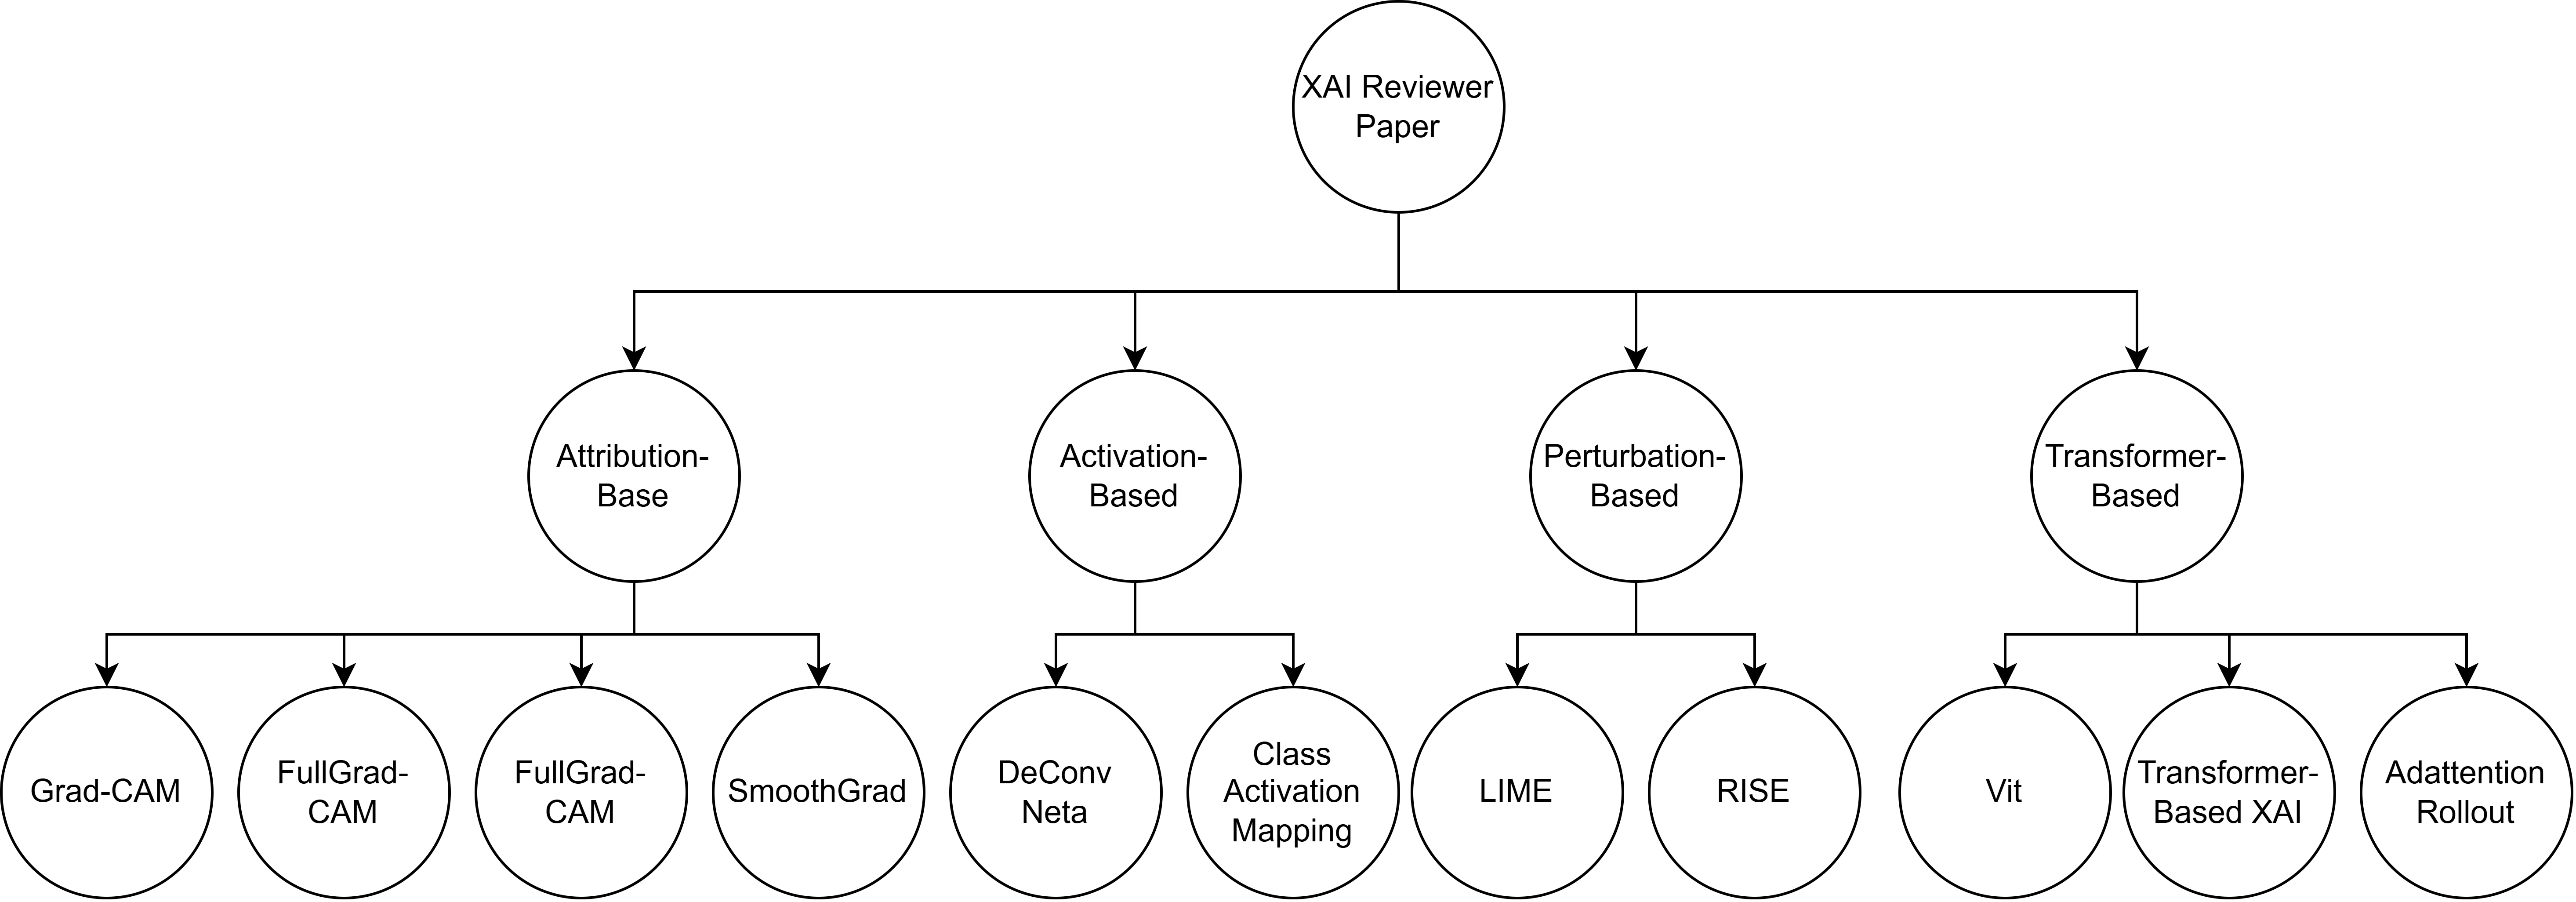
\includegraphics[width=0.7\textwidth]{images/HierarkiXAI.png}
	\caption{Kategorisasi hierarkis metode XAI \autocite{iftikhar2025explainable}}
	\label{gambar:hierarkiXAI}
\end{figure}

\textit{Attribution-based methods} memiliki konsep dengan memberi nilai pada setiap bagian masukan gambar. Bagian yang paling memengaruhi keputusan akhir akan mendapat nilai tinggi. Hal ini dapat membantu penggunanya untuk melihat area pada gambar yang paling penting bagi AI. \textit{Activation-based methods} melihat bagian gambar yang membuatnya bereaksi untuk memberikan penjelasan bagaimana AI mengenali fitur gambar secara bertahap. \textit{Perturbation-based methods} menjelaskan keputusan dengan memodifikasi atau melakukan \textit{masking} sebagian masukan dan mengamati dampaknya pada keluaran. \textit{Transformer-based methods} memanfaatkan mekanisme \textit{self-attention} dari \textit{vision transformers} dan model terkait sehingga bisa menunjukkan bagian gambar yang sedang fokus diperhatikan oleh AI saat mengambil keputusan \autocite{iftikhar2025explainable}.

\subsubsection{\textit{Attribution-based Methods}}
\textit{Attribution-based methods} menghasilkan visualisasi seperti \textit{heatmap} dengan cara melacak representasi internal model, seperti gradien atau aktivasi, secara mundur dari \textit{output} prediksi ke \textit{input}. Metode ini memiliki asumsi bahwa tingkat kepentingan sebuah fitur \textit{input} dapat diturunkan dari bagaimana perubahan pada fitur tersebut memengaruhi \textit{output} akhir model. Terdapat beberapa algoritma \textit{attribution-based methods} \autocite{iftikhar2025explainable}, yaitu:

\begin{enumerate}
	\item \textit{Gradient-weighted Class Activation Mapping} (Grad-CAM)\\
	Grad-CAM adalah sebuah metode XAI yang digunakan untuk memahami pentingnya berbagai lapisan dan fitur dalam sebuah CNN. Fungsi utamanya adalah membantu menemukan wilayah pada sebuah gambar yang memiliki dampak terbesar terhadap prediksi model.
	
	\item FullGrad-CAM dan FullGrad-CAM++\\
	Metode FullGrad-CAM dan FullGrad-CAM++ memperluas Grad-CAM dengan menggabungkan semua kontribusi bias dan gradien dari lapisan-lapisan sebelumnya. FullGrad-CAM melakukan \textit{backpropagate gradient} dan mengakumulasi nilai absolutnya untuk menghasilkan penjelasan yang lebih informatif. 
	
	\item SmoothGrad\\
	SmoothGrad mengurangi \textit{visual noise} dengan menambahkan \textit{Gaussian perturbation} kecil ke masukan beberapa kali dan mengambil rata-rata penjelasan berbasis gradien dari variasi-variasi ini. Hal ini dapat menghaluskan perubahan nilai yang sangat drastis yang muncul dalam metode berbasis gradien.
	
\end{enumerate}

\subsubsection{\textit{Perturbation-based Methods}}
\textit{Perturbation-based methods} menjelaskan prediksi model dengan sengaja mengubah \textit{input} dan mengamati bagaimana \textit{output}-nya berubah. Saat sebuah bagian dari \textit{input} ditutupi, diubah, atau dihilangkan dan menyebabkan prediksi model berubah drastis, bagian tersebut akan dianggap penting bagi keputusan model. Terdapat beberapa algoritma \textit{perturbation-based methods} \autocite{iftikhar2025explainable}, yaitu:

\begin{enumerate}
	\item 	LIME (\textit{Local Interpretable Model-Agnostic Explanations})\\
	Metode LIME membagi \textit{input} menjadi segmen-segmen yang dapat ditafsirkan lalu mengganggu segmen-segmen ini dengan menyalakan atau mematikannya secara acak dan melatih model lokal yang lebih sederhana untuk meniru keputusan model \textit{black-box} hanya di area tersebut. Bobot atau tingkat kepentingan dari model ini yang digunakan untuk menjelaskan fitur yang paling penting.
	
	
	\item RISE (\textit{Randomized Input Sampling for Explanation})\\
	Metode RISE bekerja dengan membuat banyak \textit{mask} biner secara acak yang menutupi bagian-bagian gambar. Setiap gambar yang ditutupi \textit{mask} dimasukkan ke model untuk dilihat skor prediksinya. Setelah itu, peta yang menunjukkan bagian penting dihasilkan dengan menggabungkan semua \textit{mask} acak tersebut.
	
\end{enumerate}

\subsubsection{\textit{Activation-based Methods}}
\textit{Activation-based methods} adalah teknik yang menghasilkan penjelasan dengan cara melihat langsung \textit{feature maps} di dalam lapisan-lapisan jaringan saraf (CNN). Terdapat beberapa algoritma \textit{activation-based methods} \autocite{iftikhar2025explainable}, yaitu:


\begin{enumerate}
	\item DeConvNets (\textit{Deconvolutional Networks})\\
	Metode DeConvNets memiliki tujuan untuk memahami dan memvisualisasikan apa yang telah dipelajari oleh setiap neuron atau lapisan dalam sebuah CNN. Metode DeConvNets mengambil sebuah aktivasi fitur dari lapisan dalam seperti neuron yang aktif dan merekonstruksinya kembali ke ruang \textit{input}. Hasil dari metode ini adalah sebuah gambar yang menunjukkan pola visual yang membuat neuron tersebut aktif.
	
	\item \textit{Class Activation Mapping} (CAM)\\
	Metode CAM dilakukan untuk mengidentifikasi wilayah pada gambar \textit{input} yang paling penting yang digunakan model untuk membuat prediksi kelas tertentu. CAM melihat \textit{importance weights} dari lapisan \textit{global average pooling} yang terletak tepat sebelum lapisan keputusan akhir. Setelah itu, CAM menyorot area pada gambar asli yang memiliki peta fitur penting aktif. Hasilnya adalah sebuah \textit{heatmap} yang menunjukkan lokasi bukti. 
	
\end{enumerate}

\subsubsection{\textit{Transformer-based Methods}}
\textit{Transformer-based methods} merupakan metode khusus pada arsitektur \textit{Vision Transformer} (ViT) yang berfokus pada mekanisme \textit{attention} bawaan dari model itu sendiri. ViT memproses gambar dengan membaginya menjadi beberapa potongan dan kemudian menghitung skor atensi di antara semua \textit{patch} tersebut. Teknik ini mengekstrak dan memvisualisasikan skor atensi ini untuk menghasilkan peta yang menunjukkan bagian gambar yang paling diperhatikan oleh model saat mengambil keputusan \autocite{iftikhar2025explainable}.

\section{Evaluasi}
Evaluasi model \textit{deep learning} sangat krusial untuk menilai kemampuan nyata model dalam menggeneralisasi data baru, bukan sekadar melihat seberapa kecil tingkat kesalahan saat pelatihan. Metrik performa adalah alat ukur yang jauh lebih mudah diinterpretasikan untuk membandingkan secara objektif dan memilih konfigurasi model yang paling optimal. Oleh karena itu, evaluasi wajib disesuaikan dengan tantangan spesifik masing-masing tugas untuk memastikan bahwa model terbukti akurat dan dapat diandalkan saat menghadapi skenario di dunia nyata \autocite{terven2025survey}.

\subsection{\textit{Deep Learning}}
\label{sec:Deep Learning}
Salah satu komponen penting dari \textit{deep learning} untuk melatih dan mengevaluasi model adalah \textit{performance metrics}. \textit{Performance metrics} menilai kemampuan model untuk membuat prediksi akurat pada data yang belum pernah dilihat. Berdasarkan \textcite{wozniak2021deep}, terdapat beberapa \textit{performance metrics} yang digunakan dalam pendeteksian tumor otak menggunakan \textit{deep learning}, yaitu:
\begin{enumerate}
	\item Akurasi (\textit{Accuracy}) \\
	Mengukur rasio prediksi benar secara keseluruhan dengan membandingkan prediksi positif dan negatif yang benar (\textit{True Positives} dan \textit{True Negatives}) terhadap total seluruh data.
	\item Presisi (\textit{Precision}) \\
	Mengukur ketepatan prediksi positif yang dihasilkan oleh model, yaitu proporsi prediksi tumor yang benar-benar merupakan tumor dari keseluruhan prediksi positif yang dihasilkan model.
	\item \textit{Recall} \\
	Mengukur kemampuan model dalam menemukan semua sampel positif (kasus tumor) yang sebenarnya ada di dalam data, atau dikenal juga sebagai \textit{sensitivity}.
	\item Spesifisitas (\textit{Specificity}) \\
	Mengukur kemampuan model dalam mengidentifikasi hasil negatif (kasus non-tumor/sehat) dengan benar. \textcite{wozniak2021deep} menunjukkan bahwa metrik ini penting dalam konteks medis karena mencerminkan seberapa rendah kecenderungan model salah mengklasifikasikan pasien sehat sebagai penderita tumor, sehingga meningkatkan keandalan model saat diterapkan pada pemeriksaan klinis.
	\item \textit{F1-Score} \\
	Mengukur keseimbangan model menggunakan rata-rata harmonik dari \textit{Precision} dan \textit{Recall}, sehingga cocok digunakan ketika distribusi kelas data tidak seimbang.
\end{enumerate}

Kelima metrik tersebut digunakan secara bersamaan oleh \textcite{wozniak2021deep} untuk mengevaluasi model \textit{Correlation Learning Mechanism} (CLM) pada deteksi tumor otak berbasis citra CT scan.

\subsection{\textit{Explainable Artificial Intelligence} (XAI)}
Berdasarkan \textcite{kadir2023evaluation}, untuk melakukan evaluasi terhadap XAI, diperlukan metrik XAI yang bisa ditentukan oleh dua taksonomi, yaitu taksonomi berbasis aplikasi dan taksonomi berbasis metodologi evaluasi.

\begin{enumerate}
	\item Taksonomi Berbasis Aplikasi \\
	Taksonomi berbasis aplikasi adalah klasifikasi yang mengelompokkan metrik XAI berdasarkan tujuan konseptualnya. Hal ini memisahkan konsep umum seperti \textit{user satisfaction} dan \textit{transparency} dari metode \textit{local explanation} yang lebih teknis beserta turunannya seperti \textit{attribution} dan \textit{saliency} \autocite{kadir2023evaluation}.
	
	\begin{figure}[H]
		\centering
		\captionsetup{justification=centering}
		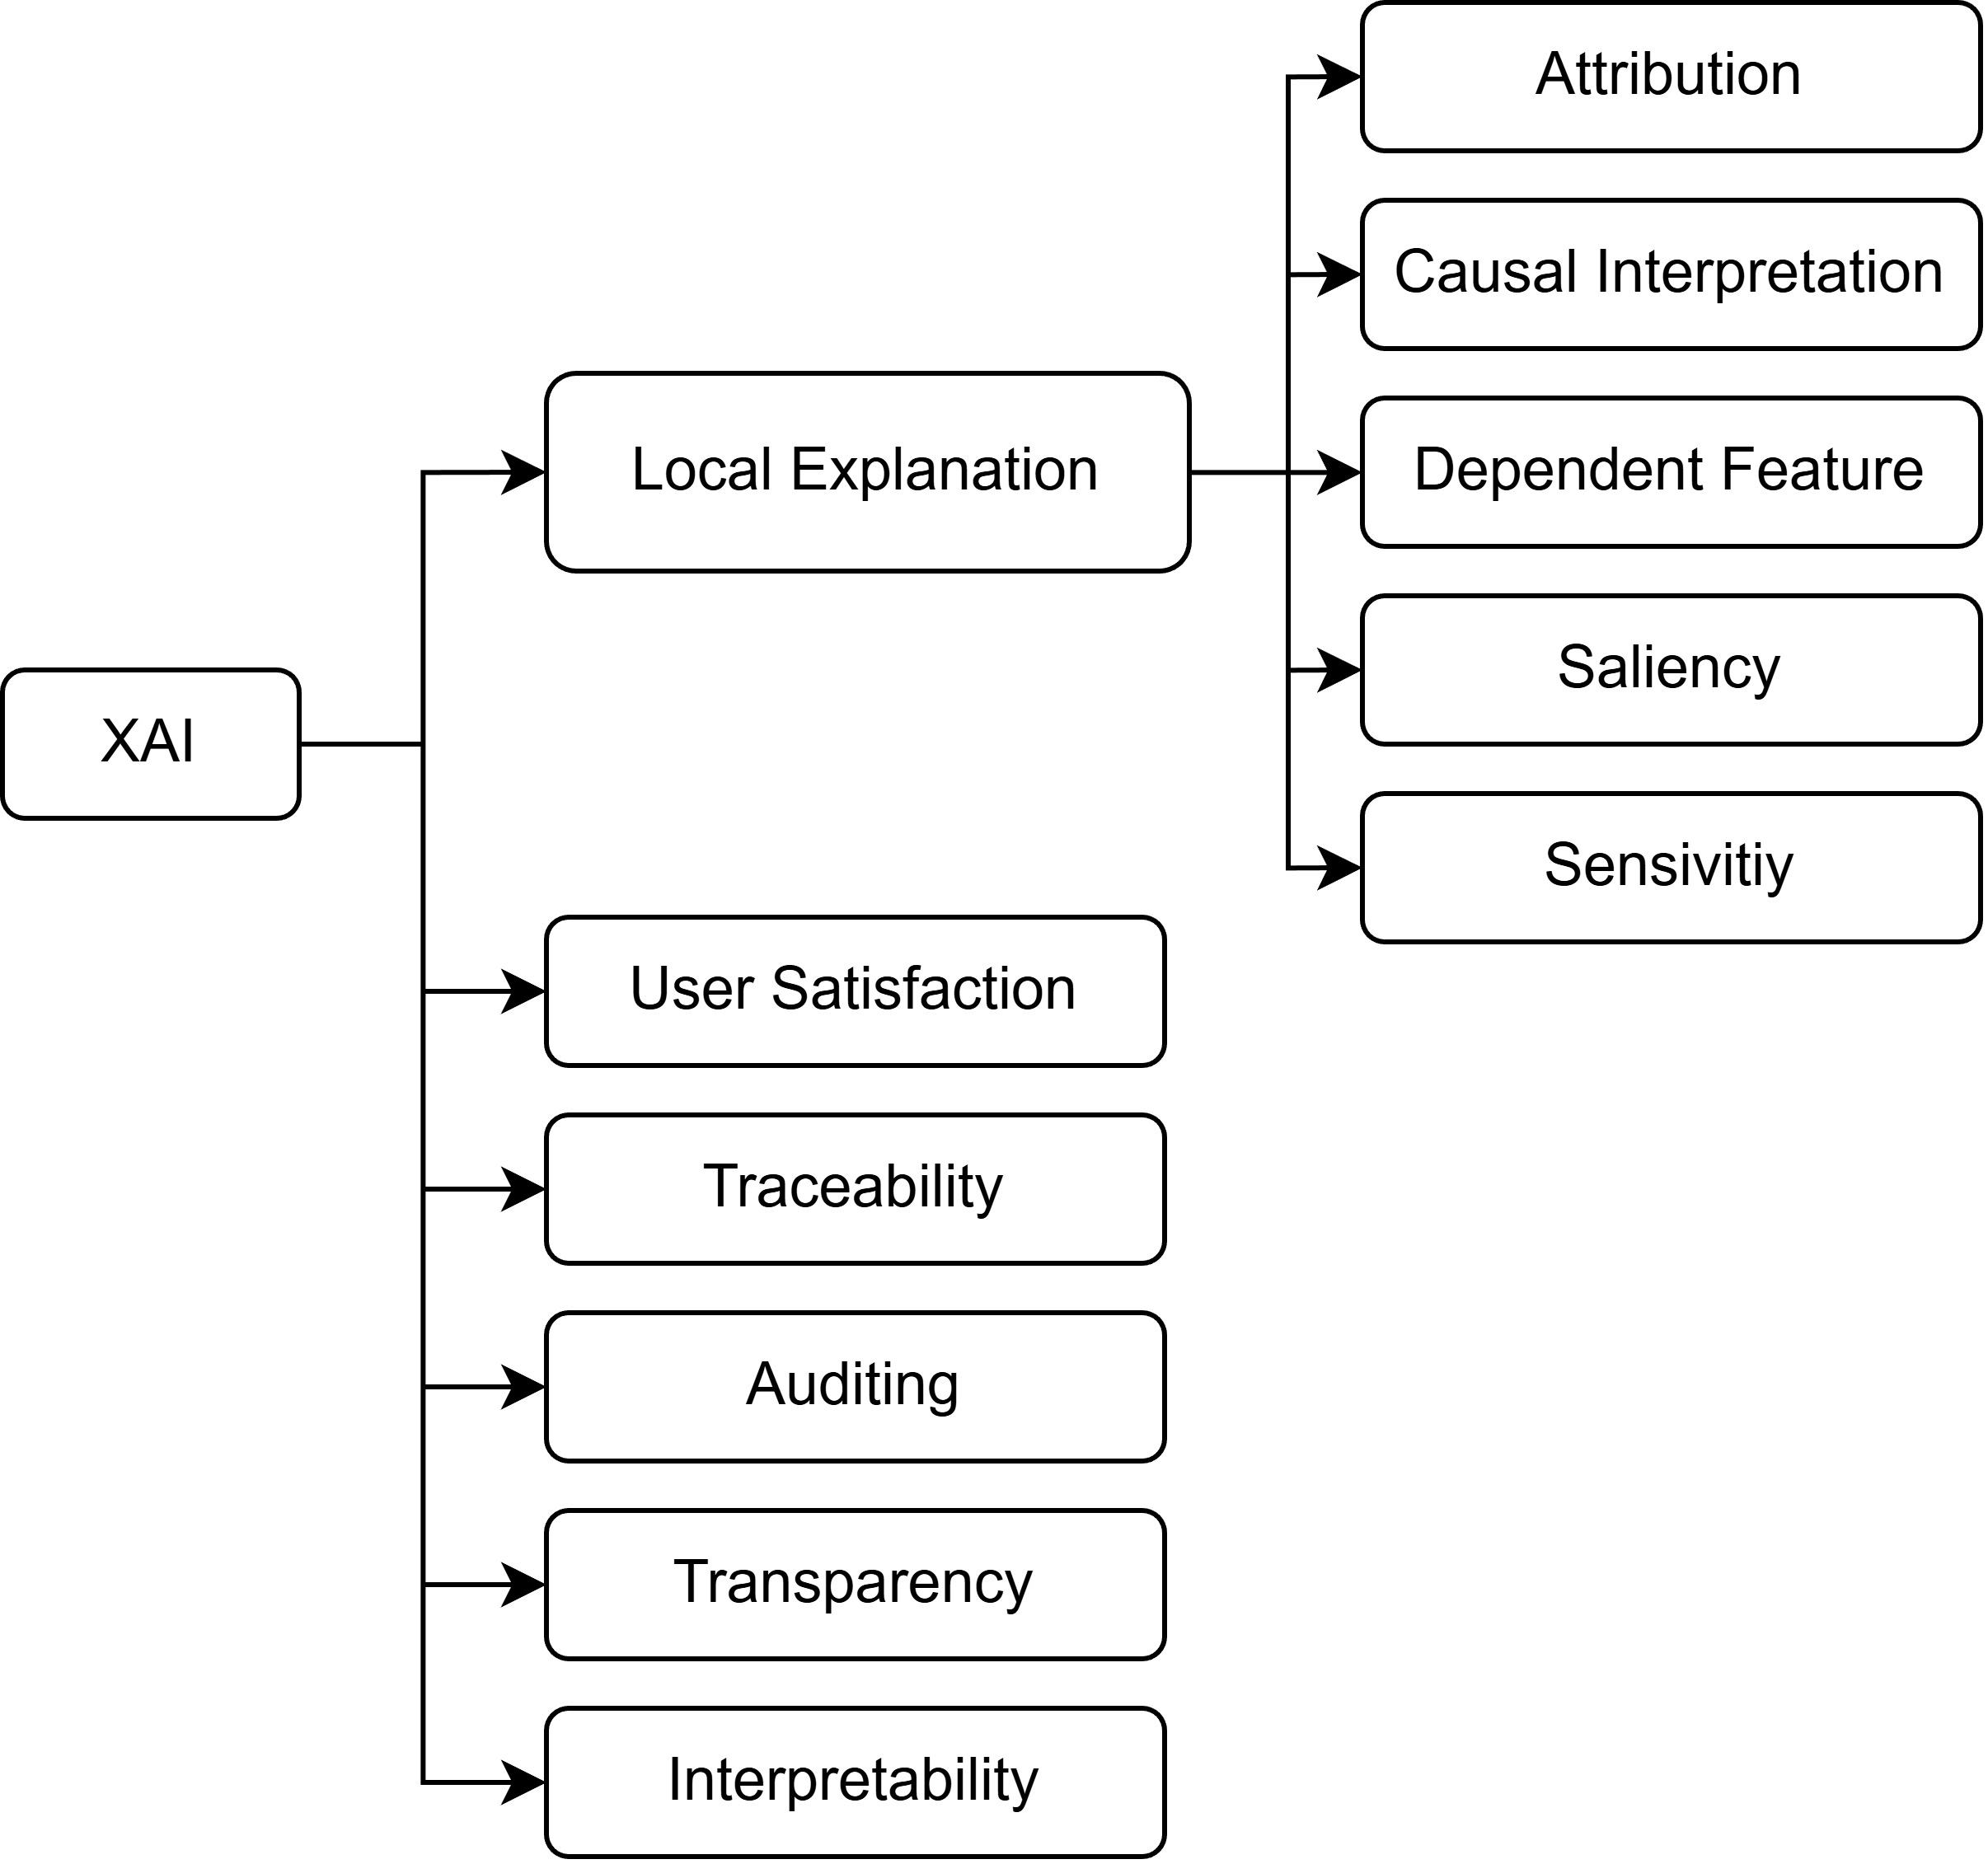
\includegraphics[width=0.7\textwidth]{images/TaksonomiXAI.png}
		\caption{Taksonomi berdasarkan aplikasi XAI \autocite{kadir2023evaluation}}
		\label{gambar:taksonomiXAI}
	\end{figure}
	
	\item Taksonomi Berbasis Metodologi Evaluasi \\
	Taksonomi berbasis metodologi evaluasi mengklasifikasikan teknik-teknik evaluasi penjelasan lokal ke dalam tiga pendekatan teknis utama, yaitu \textit{retraining}, \textit{ground truth comparison}, dan \textit{input perturbation} \autocite{kadir2023evaluation}. 
	
	\begin{figure}[H]
		\centering
		\captionsetup{justification=centering}
		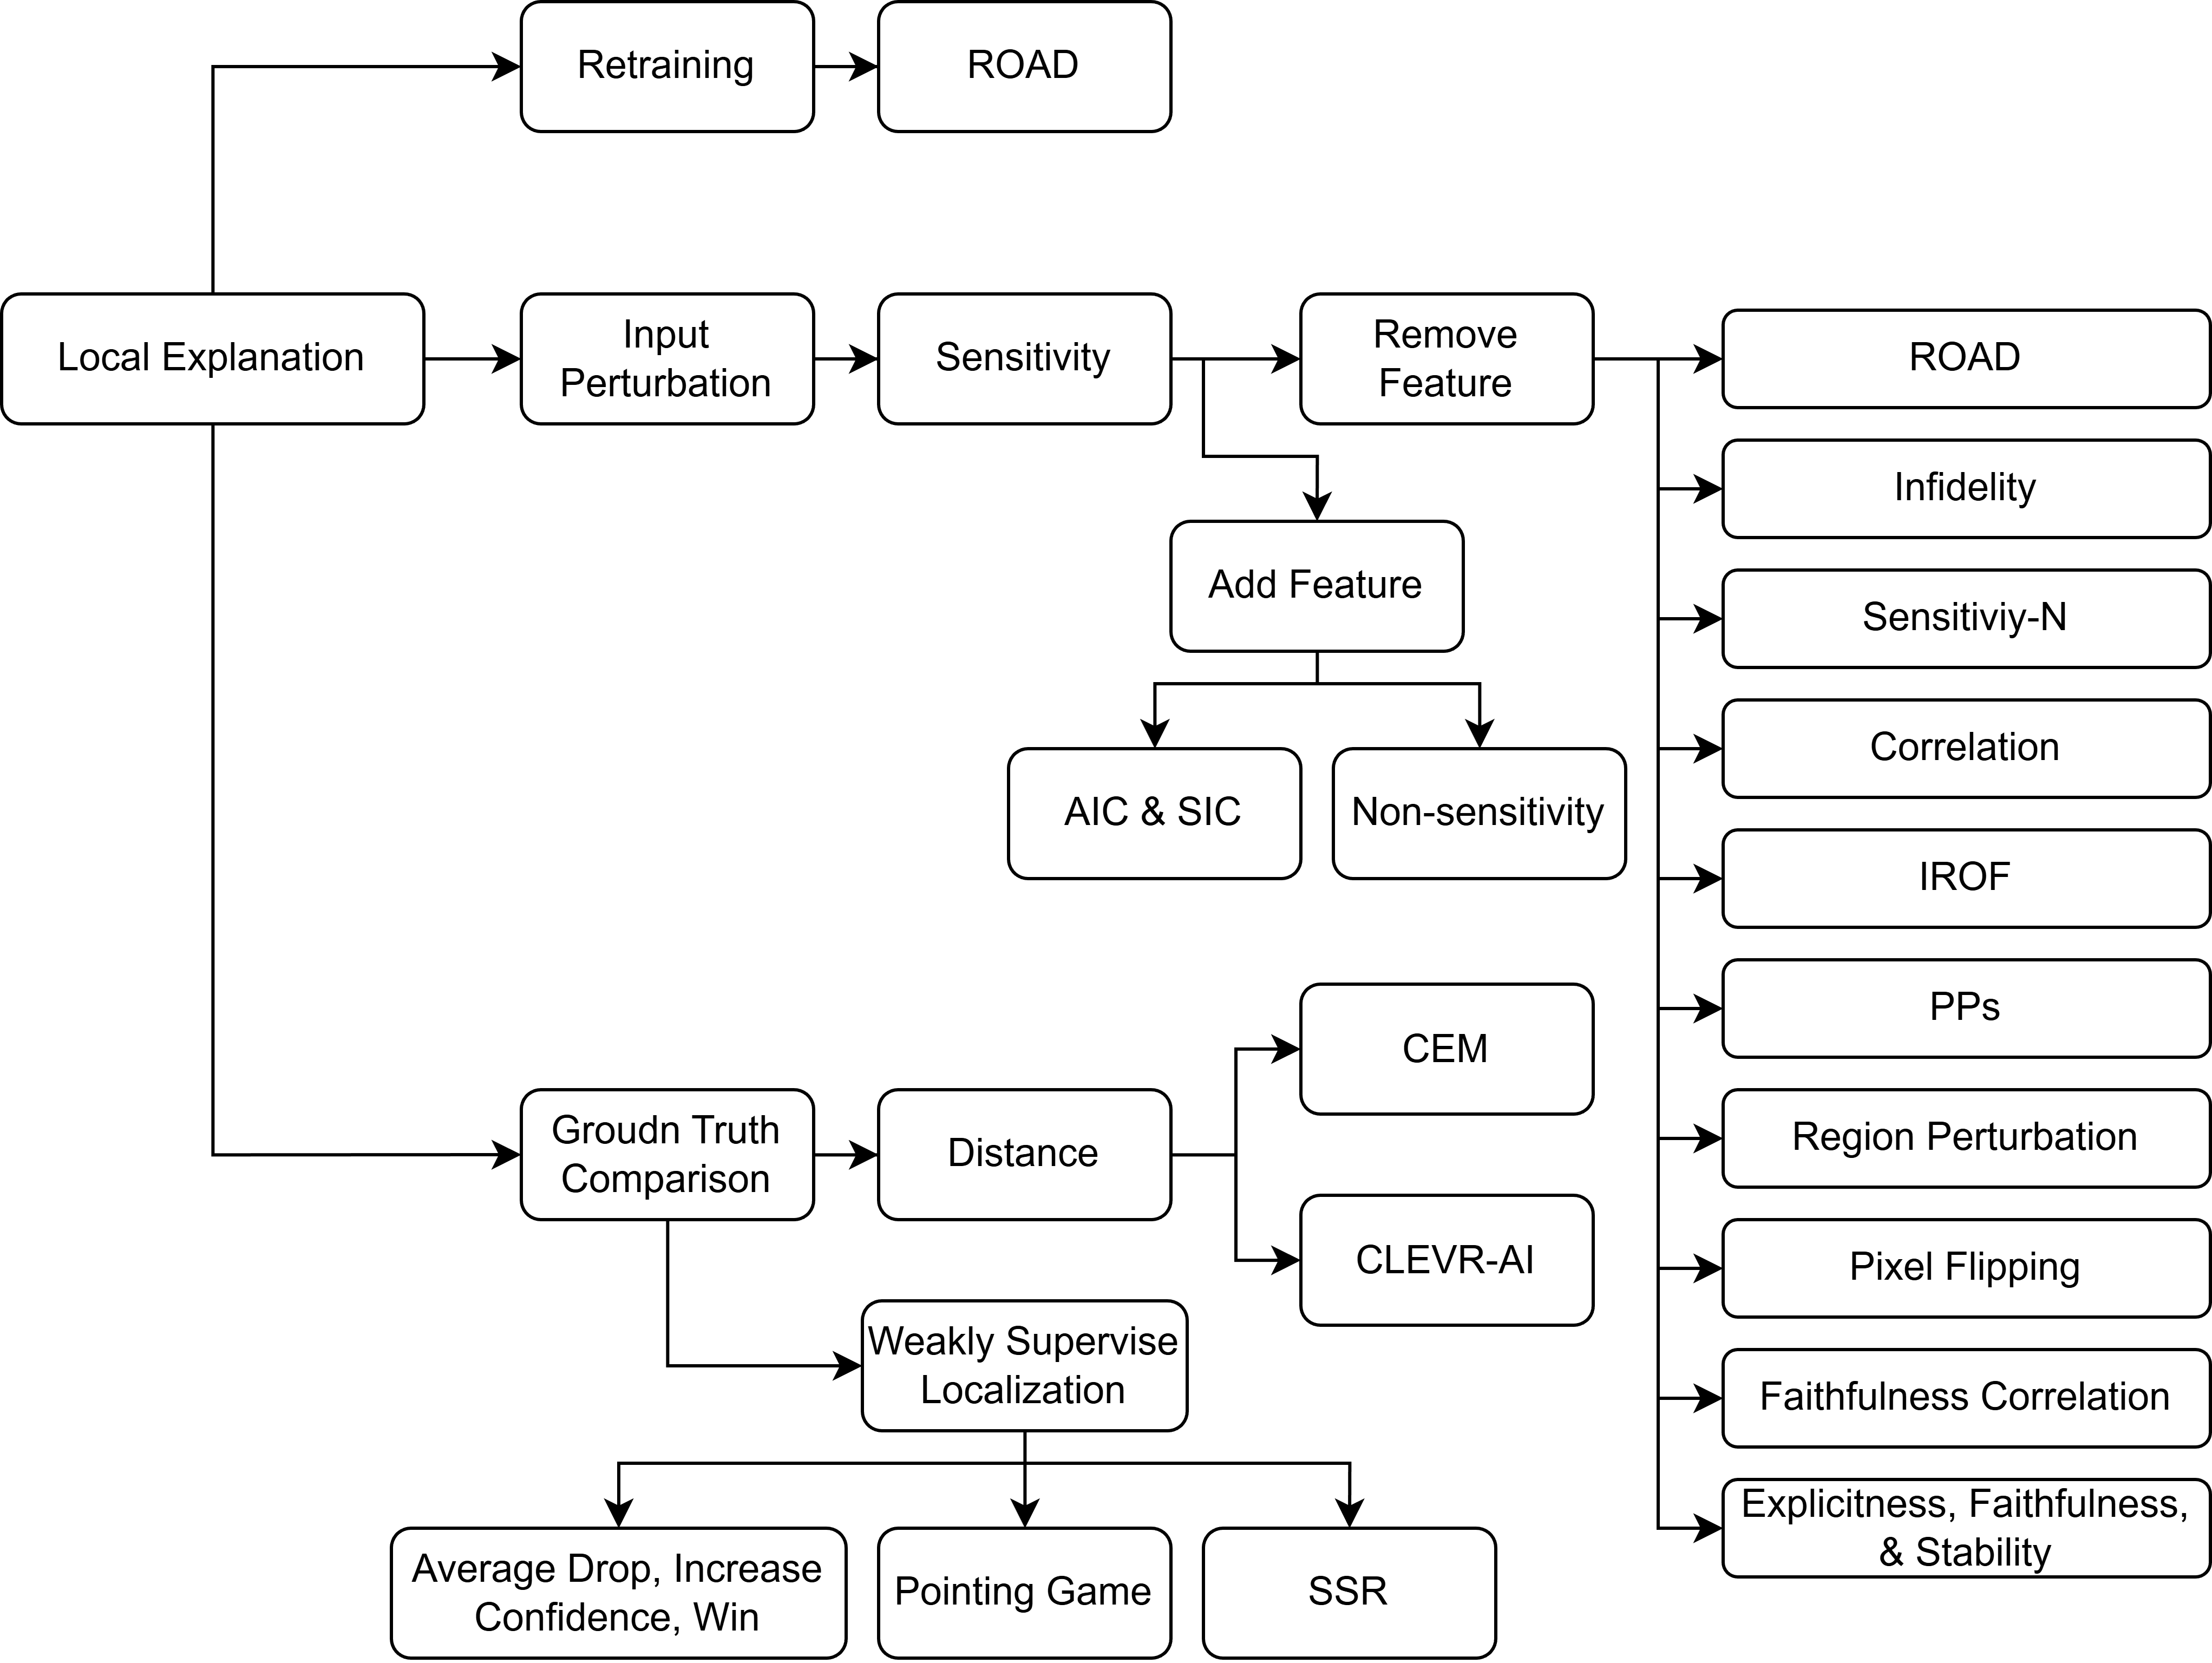
\includegraphics[width=0.7\textwidth]{images/TaksonomiXAI2.png}
		\caption{Taksonomi berdasarkan metodologi evaluasi \autocite{kadir2023evaluation}}
		\label{gambar:taksonomiXAI2}
	\end{figure}
	
	Dalam pendekatan \textit{ground truth comparison}, terdapat penelitian terbaru oleh \textcite{muhammad2025heatmap} yang mengusulkan metrik evaluasi kuantitatif bernama XAlign. Metrik ini dirancang untuk mengatasi keterbatasan metrik yang tumpang tindih standar dengan menilai \textit{spatial fidelity heatmap} melalui tiga komponen integratif yang diformulasikan sebagai berikut.
	
	\begin{enumerate}
		\item \textit{Weighted Relevance Overlap} (WRO) \\
		Komponen ini mengukur proporsi relevansi penjelasan yang terlokalisasi secara tepat di dalam area anotasi ahli. Semakin tinggi nilai WRO, semakin fokus penjelasan tersebut pada area klinis yang relevan. Secara matematis, WRO didefinisikan seperti pada Persamaan \ref{eq:wro}:
		\begin{equation}
			WRO = \frac{\sum_{i \in G} X_{i}}{\sum_{i} X_{i}}
			\label{eq:wro}
		\end{equation}
		\eqcaption{\textit{Weighted Relevance Overlap}}
		$G$ merepresentasikan himpunan piksel dalam masker \textit{ground truth}. $X_i$ adalah skor relevansi intensitas \textit{heatmap} pada piksel ke-$i$.
		
		\item \textit{Boundary Agreement Score} (BAS) \\
		BAS menilai ketepatan penyelarasan struktural antara batas \textit{heatmap} dengan kontur lesi atau tumor menggunakan \textit{Hausdorff Distance} yang dinormalisasi, seperti yang ditunjukkan pada Persamaan \ref{eq:bas}:
		\begin{equation}
			BAS = 1 - \frac{HD(G, X)}{\text{max\_dim}(I)}
			\label{eq:bas}
		\end{equation}
		\eqcaption{\textit{Boundary Agreement Score}}
		$HD(G, X)$ adalah jarak Hausdorff antara kontur \textit{ground truth} ($G$) dan peta penjelasan ($X$). $max\_dim(I)$ adalah dimensi maksimum citra untuk normalisasi. Nilai BAS yang mendekati 1 mengindikasikan korespondensi anatomis yang presisi.
		
		\item \textit{Dispersion Penalty} (DP) \\
		Komponen ini memberikan penalti terhadap penyebaran atribusi di luar area klinis untuk memastikan peta \textit{saliency} tetap ringkas, dengan formulasi pada Persamaan \ref{eq:dp}:
		\begin{equation}
			DP = \frac{\sum_{i \notin G} X_{i}}{\sum_{i} X_{i}}
			\label{eq:dp}
		\end{equation}
		\eqcaption{\textit{Dispersion Penalty}}
		$i \notin G$ menunjukkan piksel yang berada di luar area \textit{ground truth}. Nilai DP yang lebih rendah menandakan penjelasan yang lebih fokus dengan sedikit \textit{noise} latar belakang.\\
	\end{enumerate}
	
	Secara keseluruhan, skor akhir XAlign dihitung dengan menggabungkan ketiga komponen tersebut menggunakan bobot skalar ($\alpha, \beta, \gamma$) seperti pada Persamaan \ref{eq:xalign}:
	\begin{equation}
		XAlign = \alpha \cdot WRO + \beta \cdot BAS - \gamma \cdot DP
		\label{eq:xalign}
	\end{equation}
	\eqcaption{XAlign}
	Penggunaan XAlign memungkinkan evaluasi yang tidak hanya mengukur akurasi lokasi, tetapi juga kepatuhan bentuk penjelasan terhadap anatomi tumor yang sebenarnya \autocite{muhammad2025heatmap}.
\end{enumerate}

Untuk menentukan metrik evaluasi XAI, prosesnya dimulai dengan mengidentifikasi konsep yang akan diuji menggunakan taksonomi berbasis aplikasi. Taksonomi ini membantu membedakan apakah tujuannya adalah untuk mengukur konsep umum seperti \textit{user satisfaction} dan \textit{transparency}, atau untuk mengevaluasi penjelasan teknis yang lebih spesifik seperti \textit{local explanation}, yang mencakup metode seperti \textit{saliency}. Setelah itu, taksonomi berbasis metodologi evaluasi digunakan untuk memilih pendekatan teknis yang sesuai untuk mengevaluasi penjelasan lokal tersebut \autocite{kadir2023evaluation}.

\section{Penelitian Terkait Pendeteksian Tumor}
\label{sec:penelitian terkait tumor}
Pendeteksian dan klasifikasi tumor otak merupakan salah satu topik yang terus berkembang dalam bidang pengolahan citra medis, seiring dengan semakin banyaknya penerapan metode \textit{deep learning} untuk membantu proses diagnosis. Berbagai penelitian telah dilakukan dengan memanfaatkan citra \textit{CT Scan} maupun MRI menggunakan pendekatan yang beragam, mulai dari kombinasi fitur \textit{handcrafted} dengan \textit{deep learning}, optimasi arsitektur CNN, hingga penerapan \textit{explainable AI} (XAI) untuk meningkatkan interpretabilitas model. Pada bagian ini akan dibahas beberapa penelitian terkait yang menjadi acuan dalam tugas akhir ini, beserta kelebihan dan kekurangan dari masing-masing pendekatan yang digunakan.

\subsubsection{\textit{Detection and Classification of Brain Tumor Using a Hybrid Learning Model in CT Scan Images}} \label{subsubsec:hybrid_tumor}
\textcite{ghasemi2025detection} mengajukan model hibrid yang menggabungkan fitur \textit{handcrafted} (LBP, HOG, dan intensitas median) dengan fitur \textit{deep learning} dari ResNet50 dan AlexNet yang dioperasikan dalam mode \textit{frozen}, diseleksi menggunakan algoritma SelectKBest ($k = 10.000$), dan diklasifikasikan melalui \textit{Multilayer Perceptron} (MLP) lima lapisan untuk membedakan empat kelas tumor otak pada citra \textit{CT Scan}. Meskipun pendekatan fusi fitur ini terbukti efektif dengan akurasi 94,82\%, spesifisitas 98,35\%, dan AUC $> 0,98$ pada seluruh kelas, terdapat sejumlah kelemahan mendasar yang perlu dicermati. \textit{Dataset} yang digunakan hanya bersumber dari satu repositori daring (Radiopaedia) dengan total 1.388 citra, sehingga generalisabilitas model ke skenario klinis multisenter masih dipertanyakan. Selain itu, penggunaan CNN \textit{pre-trained} tanpa \textit{fine-tuning} berpotensi membatasi adaptasi model terhadap karakteristik spesifik citra CT otak, mengingat bobot yang digunakan dilatih pada \textit{domain} ImageNet yang berbeda secara signifikan. Ketiadaan analisis \textit{explainability} juga menjadi hambatan adopsi klinis yang krusial.

\subsubsection{\textit{Deep Neural Network Correlation Learning Mechanism for CT Brain Tumor Detection}}
\label{subsubsec:CLM}
\textcite{wozniak2021deep} mengajukan \textit{Correlation Learning Mechanism} (CLM) yang mengintegrasikan CNN dengan ANN klasik untuk mendeteksi tumor otak pada citra \textit{CT Scan} secara adaptif. Inovasi utamanya terletak pada mekanisme pemilihan palet filter secara dinamis, yaitu ANN mengevaluasi hasil CNN dan menyimpan konfigurasi terbaik ke dalam arsip untuk menyempurnakan iterasi berikutnya. Proses pelatihan dipercepat melalui implementasi \textit{multi-threading} paralel berbasis algoritma Adam, yang memungkinkan eksplorasi ruang konfigurasi secara luas dalam waktu singkat. Model dievaluasi pada dua \textit{dataset} citra CT dan mencapai akurasi 96,55\% serta 95,09\%, dengan spesifisitas 97,43\% sebagai nilai tertinggi dibandingkan metode pembanding, mengindikasikan kemampuan superior dalam meminimalkan diagnosis positif palsu.

\subsubsection{\textit{Explainable CNN for brain tumor detection and classification through XAI based key features identification}}
\label{subsubsec:expcnn}
\textcite{Iftikhar2025ExplainableCNN} mengajukan pendekatan \textit{explainable} CNN untuk klasifikasi tumor otak guna mengatasi sifat \textit{black-box} pada model \textit{deep learning}. Penelitian ini mengintegrasikan Grad-CAM, SHAP, dan LIME ke dalam arsitektur CNN. Analisis Grad-CAM dimanfaatkan untuk memangkas \textit{layer} berkontribusi minimal sehingga menghasilkan model yang lebih efisien. Model dievaluasi pada \textit{dataset} MRI empat kelas (\textit{meningioma}, \textit{glioma}, \textit{pituitary}, \textit{no tumor}) dan mencapai akurasi 99,21\% pada data latih serta 94,72\% pada data uji, dengan visualisasi XAI yang membuktikan fokus model pada area patologis yang relevan.

\subsubsection{\textit{Deep-EFNet: An Optimized EfficientNetB0 Architecture with Dual Regularization for Scalable Multi-Class Brain Tumor Classification in MRI}}
\label{subsubsec:efnet}
\textcite{alshaari2025deepefnet} mengajukan arsitektur \textit{deep learning} berbasis \textit{transfer learning} bernama Deep-EFNet untuk klasifikasi multi-kelas tumor otak dari citra MRI, guna mengatasi tantangan kompleksitas ekstraksi fitur serta keterbatasan generalisasi model pada \textit{dataset} berukuran bervariasi. Penelitian ini memanfaatkan EfficientNetB0 sebagai \textit{backbone} pra-latih dengan bobot ImageNet, yang diperkaya dengan lapisan \textit{batch normalization}, \textit{global average pooling}, dua lapisan \textit{dense} (512 dan 256 unit dengan aktivasi ReLU dan regularisasi L2), serta \textit{dropout} bermuatan 0,5 untuk mencegah \textit{overfitting}. Pelatihan dilakukan dalam dua fase, yaitu fase pertama yang membekukan seluruh bobot \textit{backbone} dan melatih hanya \textit{classification head} dengan laju pembelajaran $10^{-4}$, serta fase kedua yang melakukan \textit{fine-tuning} pada 30 lapisan teratas dengan laju pembelajaran $10^{-3}$ agar fitur tingkat tinggi dapat diadaptasi terhadap tugas klasifikasi spesifik. Model dievaluasi pada dua \textit{dataset} MRI empat kelas (\textit{glioma}, \textit{meningioma}, \textit{pituitary}, \textit{no tumor}), yakni 3K-DS (3.064 citra) dan 7K-DS (7.023 citra), menggunakan validasi \textit{5-fold cross-validation}. Hasil menunjukkan akurasi 95,4\% pada 3K-DS dan 98,2\% pada 7K-DS untuk evaluasi \textit{single-split}, serta ROC-AUC sebesar 0,99-1,00 di seluruh kelas, melampaui metode mutakhir seperti \textit{hybrid} CNN (94\%), CGAN (97\%), dan Deep-GAN (96\%).

\subsection{Penelitian Terkait XAI}
Seiring dengan meningkatnya penggunaan model \textit{deep learning} untuk mendeteksi tumor otak, muncul pula tantangan baru berupa kurangnya transparansi dalam proses pengambilan keputusan model tersebut, yang dikenal sebagai sifat \textit{black-box}. Kondisi ini menjadi perhatian penting karena tenaga medis memerlukan alasan yang jelas di balik suatu prediksi sebelum dapat mempercayai dan menggunakannya sebagai alat bantu diagnosis. Untuk mengatasi permasalahan tersebut, sejumlah penelitian mengintegrasikan teknik \textit{Explainable AI} (XAI) seperti Grad-CAM, SHAP, dan LIME ke dalam model klasifikasi tumor otak guna memberikan visualisasi maupun penjelasan yang lebih mudah dipahami mengenai dasar prediksi yang dihasilkan model.

\subsubsection{\textit{An XAI-Enhanced EfficientNetB0 Framework for Precision Brain Tumor Detection in MRI Imaging}}

\textcite{mahesh2024xai} mengintegrasikan teknik \textit{Explainable AI} (XAI) berupa \textit{Gradient-weighted Class Activation Mapping} (Grad-CAM) ke dalam model klasifikasi tumor otak berbasis MRI, dengan tujuan mengatasi sifat \textit{black-box} model \textit{deep learning} yang menghambat kepercayaan tenaga medis terhadap rekomendasi diagnostik berbasis AI. Grad-CAM bekerja dengan menghitung gradien kelas keluaran terhadap peta fitur lapisan konvolusi terakhir, menghasilkan \textit{heatmap} yang divisualisasikan di atas citra MRI untuk menunjukkan area yang paling memengaruhi prediksi model. Penelitian ini mengklaim bahwa pola \textit{heatmap} yang dihasilkan selaras dengan penanda diagnostik klinis yang sudah dikenal, seperti lokalisasi massa tumor pada kasus \textit{glioma} dan aktivasi yang menyebar pada kasus \textit{No Tumor}.

\subsubsection{\textit{Explainable CNN for Brain Tumor Detection and Classification through XAI Based Key Features Identification}}

\textcite{Iftikhar2025ExplainableCNN} mengajukan pendekatan CNN berbasis XAI untuk klasifikasi tumor otak multi-kelas dari citra MRI. Grad-CAM dimanfaatkan tidak hanya sebagai alat visualisasi, tetapi juga sebagai mekanisme pemangkasan arsitektur model secara sistematis dengan mengeliminasi lapisan-lapisan yang berada di bawah ambang batas kontribusi minimum, sehingga menghasilkan model yang lebih ringkas tanpa penurunan performa yang signifikan. Validasi interpretabilitas dilengkapi dengan SHAP untuk analisis kepentingan fitur secara global dan LIME untuk eksplanasi berbasis \textit{superpixel} pada level prediksi individual. Model dievaluasi pada dua \textit{dataset} MRI empat kelas dengan total 7.023 citra (Msoud) dan 3.264 citra (NeuroMRI), mencapai akurasi 99,21\% pada data \textit{seen} dan 94,72\% pada data \textit{unseen}. Keterbatasan utama studi ini adalah cakupan evaluasi yang terbatas pada modalitas MRI tanpa validasi silang pada modalitas pencitraan lain seperti \textit{CT Scan}, serta belum dilakukannya validasi klinis formal oleh tenaga medis. Celah ini menjadi salah satu landasan tugas akhir untuk mengeksplorasi penerapan integrasi XAI pada modalitas \textit{CT Scan} yang lebih umum tersedia di fasilitas kesehatan Indonesia.

\section{Kesenjangan Penelitian}
Meskipun penelitian di bidang deteksi dan klasifikasi tumor berbasis \textit{deep learning} telah menunjukkan perkembangan yang pesat, sejumlah kesenjangan mendasar masih belum tertangani secara memadai dalam literatur yang ada.

Pertama, sebagian besar penelitian masih terfokus pada modalitas MRI dan belum memvalidasi pendekatan mereka pada \textit{CT Scan}. \textcite{alshaari2025deepefnet} hanya mengevaluasi Deep-EFNet pada dua \textit{dataset} MRI tanpa eksplorasi lintas modalitas, sementara \textcite{Iftikhar2025ExplainableCNN} juga membatasi evaluasinya secara eksklusif pada MRI meskipun arsitekturnya dirancang untuk klasifikasi multi-kelas yang lebih general. \textit{CT Scan} memiliki karakteristik intensitas, resolusi kontras, dan artefak yang secara fundamental berbeda dari MRI, sehingga kemampuan model maupun interpretabilitas XAI yang telah terbukti pada MRI tidak dapat diasumsikan berlaku langsung pada modalitas ini. Padahal, \textit{CT Scan} merupakan modalitas yang jauh lebih tersedia dan terjangkau di fasilitas kesehatan negara berkembang, termasuk Indonesia, sehingga validasi pada modalitas ini menjadi kebutuhan yang mendesak secara klinis.

Kedua, terdapat kesenjangan yang tidak homogen dalam hal adopsi \textit{explainability}, yaitu sebagian penelitian yang sama sekali tidak menyertakan komponen XAI dan sebagian lainnya yang telah mengadopsinya namun masih dalam lingkup validasi yang dangkal. \textcite{alshaari2025deepefnet} tidak mengintegrasikan teknik XAI apapun sehingga proses pengambilan keputusan model sepenuhnya bersifat \textit{black-box} dan menyulitkan interpretasi klinis. Kondisi serupa dijumpai pada \textcite{ghasemi2025detection} yang mengusulkan model hibrid berbasis \textit{CT Scan} dengan akurasi kompetitif, namun tidak menyertakan mekanisme \textit{explainability} apapun. Arsitektur fusi fitur yang kompleks justru memperparah sifat \textit{black-box}-nya karena kontribusi masing-masing komponen fitur (LBP, HOG, ResNet50, maupun AlexNet) terhadap keputusan klasifikasi tidak dapat ditelusuri secara transparan, sehingga klaim potensi klinis yang diajukan penulis sulit dipertanggungjawabkan tanpa dukungan interpretabilitas yang memadai. Di sisi lain, \textcite{mahesh2024xai} telah mengintegrasikan Grad-CAM ke dalam arsitektur EfficientNetB0, namun validasi eksplanasi yang dilakukan hanya berupa inspeksi visual terhadap kesesuaian \textit{heatmap} dengan penanda diagnostik yang sudah diketahui sebelumnya, tanpa pengukuran kuantitatif terhadap \textit{ground truth mask} tumor. Yang patut dicermati, \textcite{mahesh2024xai} sendiri mengakui dalam tinjauan literaturnya bahwa area yang disoroti Grad-CAM tidak selalu divalidasi secara klinis untuk memastikan kesesuaiannya dengan fitur yang relevan secara medis, namun metodologi yang diajukan tidak beranjak dari keterbatasan tersebut. Kondisi ini menunjukkan bahwa keberadaan teknik XAI saja tidak cukup. Validasi objektif terhadap kebermaknaan spasial eksplanasinya merupakan lapisan kebutuhan tersendiri yang masih terabaikan dalam literatur.

Berdasarkan kesenjangan-kesenjangan tersebut, tugas akhir ini mengusulkan pendekatan yang beroperasi pada modalitas \textit{CT Scan} sekaligus mengintegrasikan Grad-CAM sebagai mekanisme \textit{explainability} yang divalidasi secara objektif terhadap \textit{ground truth mask} tumor, guna menghasilkan sistem diagnosis yang tidak hanya akurat, tetapi juga transparan dan dapat dipertanggungjawabkan kesesuaian spasial eksplanasinya dalam konteks klinis yang relevan.

% dipindahkan ke analisis peluang
%\subsection{\textit{Evaluasi Klinis dan Integrasi Alur Kerja AI dalam Radiologi Diagnostik}}
%
%Dalam pengembangan model \textit{Explainable AI} (XAI) untuk deteksi tumor pada citra CT-Scan, penting untuk tidak hanya mengevaluasi metrik teknis dari algoritma, tetapi juga bagaimana model tersebut dapat dioperasionalkan di dunia nyata. Mengingat implementasi AI di bidang medis telah terbukti secara efektif, penelitian \autocite{vimalesvaran2024assessing} menawarkan kerangka kerja penting mengenai pembuktian efektivitas AI dalam alur kerja klinis. Melalui studi ACCEPT-AI, penelitian tersebut merancang uji coba acak klaster (\textit{stepped-wedge cluster randomised trial}) untuk mengevaluasi perangkat lunak qER dari Qure.ai dalam memprioritaskan interpretasi CT-Scan kepala tanpa kontras di Instalasi Gawat Darurat.
%
%Kaitan utama studi ini dengan pengembangan XAI untuk deteksi lesi atau tumor terletak pada presentasi luaran visual dari AI tersebut kepada tenaga medis. Alur pengujian dalam studi ini dibagi menjadi tiga fase berurutan: pra-implementasi, implementasi, dan pasca-implementasi. Pada fase pasca-implementasi, alur kerja AI diintegrasikan secara langsung dengan sistem rumah sakit tanpa mengubah urutan kasus secara fundamental, melainkan dengan memberikan penanda prioritas (\textit{prioritised flag}) di dalam \textit{Radiology Information System} (RIS).
%
%Alur penggunaan qER bagi dokter berjalan sebagai berikut:
%\begin{enumerate}
%	\item Ketika seorang radiolog membuka sebuah kasus dengan penanda prioritas di RIS, sistem akan menyediakan tangkapan sekunder (\textit{secondary capture}) dari qER yang ditampilkan berdampingan dengan citra asli di dalam \textit{Picture Archiving and Communication System} (PACS).
%	\item Tangkapan sekunder ini pada dasarnya berfungsi layaknya fitur interpretasi XAI, di mana sistem menampilkan kontur visual yang secara spesifik menunjukkan titik perhatian (\textit{attention point}) algoritma terhadap suatu abnormalitas (misalnya efek massa / \textit{mass effect} yang relevan dengan indikasi tumor).
%	\item Pada tahap pelaporan, radiolog tetap memegang kendali penuh atas diagnosis akhir. Mereka menggunakan pertimbangan klinis mereka sendiri untuk menyetujui temuan visual AI tersebut, memodifikasinya, atau mengabaikannya sebelum menulis dan menandatangani laporan.
%\end{enumerate}
%
%Pendekatan operasional ini memberikan perspektif bahwa luaran model AI berkinerja tinggi harus dirancang sebagai alat pendukung keputusan klinis, bukan sebagai pengganti penilaian ahli. Untuk pengembangan model XAI deteksi tumor, artikel ini menggarisbawahi bahwa efektivitas model tidak hanya diukur dari seberapa baik ia menyoroti area lesi secara terpusat, tetapi juga dari kemudahan interaksinya (seperti integrasi tangkapan sekunder berkontur ke dalam PACS) agar radiolog dapat memvalidasi penjelasan AI tersebut dengan cepat dan menurunkan waktu tunggu pelaporan.